\subsection{Opgave 44}

Grafen for en funktion f er vist på nedenstående figur.

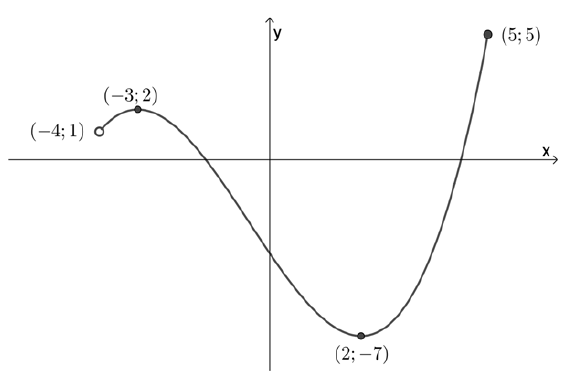
\includegraphics[width=8cm]{Opgave_41-50/Opgave_44/44.png}

Angiv funktionens monotoniforhold.

\ans

Når vi angiver en funktions monotoniforhold skal vi angive i hvilke intervaller vores funktion er voksende
og i hvilke intervaller vores funktion er aftagende.

Starter vi fra de laveste x værdier på vores funktion kan vi se at den er voksende mellem det åbne punkt $(-4; 1)$ og det lukkede punkt $(-3; 2)$ så f er voksende i intervallet
$\rbrack -4; -3 \rbrack$.

Fra det lukkede punkt $(-3; 2)$ til det lukkede punkt $(2; -7)$ er f aftagende så f er aftagende i intervallet
$[-3; 2]$.

Fra det lukkede punkt $(2; -7)$ til det lukkede punkt $(5; 5)$ er f voksende så f er voksende i intervallet $[2; 5]$.

Funktionen f har altså følgende monotoniforhold

Voksende i intervallerne: $\rbrack -4; -3\rbrack$, $[2; 5]$

Aftagende i intervallerne: $[-3; 2]$